Wenn Licht von einem Medium in ein anderes übergeht, wird es gebrochen, das heißt, es ändert seine Ausbreitungsrichtung. Die Brechung ist hauptsächlich vom Quotienten der Lichtgeschwindigkeiten in den beiden Materialien abhängig.

Allerdings spielt auch die Wellenlänge des Lichtes eine Rolle, da kurzwelliges Licht etwas stärker gebrochen wird als langwelliges. Diese Eigenschaft beruht jedoch auf komplexen Quantenphänomenen und wird nicht näher erläutert oder hergeleitet.

Das Phänomen der Brechung ist an folgendem Diagramm mit dem Huygens'schen Prinzip (\referenz{subsec:ausbreitung}) zu erklären: \footnote{„Refraction - Huygens-Fresnel principle“ von Arne Nordmann (norro) - Own illustration, based on Image:Wellen-Brechung.png and Image:Huygens\_brechung.png. Lizenziert unter CC BY-SA 3.0 über Wikimedia Commons - \url{https://commons.wikimedia.org/wiki/File:Refraction\_-\_Huygens-Fresnel\_principle.svg}}

\begin{figure}[!h]
	\center
	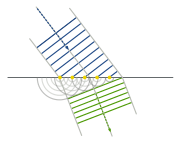
\includegraphics[width=0.7\textwidth]{brechung}
	\caption{Brechung mit dem Huygens'schen Prinzip}
	\label{fig:brechung}
\end{figure}

Die Abbildung zeigt den Übergang eines schmalen, monochromatischen (nur eine Farbe/Wellenlänge) und kohärenten (alle Elementarwellen sind Phasengleich: Siehe: \referenz{subsec:interferenz}) Lichtbündels in ein Material mit einer niedrigeren Lichtgeschwindigkeit. Ein Wellenberg löst auf der linken Seite früher Elementarwellen im neuen Medium aus als auf der rechten Seite. Da die Elementarwellen im neuen Medium langsamer sind als im alten, wird der Lichtstrahl zum Lot hin gebrochen.

\subsection{Mathematisierung}

Man denke sich nun ein senkrechtes Lot an die Kante des Materialübergangs. Die Winkel $\alpha$ sei der Winkel des Stahls im ersten Medium zum Lot und $\beta$ der Winkel des Strahls im neuen Medium zum Lot hin. Dann gilt folgendes:
	
	\begin{align}
		\frac{sin{(\alpha)}}{sin{(\beta)}} = \frac{c_1}{c_2}
	\end{align}
	
Unter Berücksichtung der Änderung der Brechung verschiedener Wellenlängen muss eine neue Größe eingeführt werden, die Brechzahl $n$, welche die Wellenlänge des Lichtes miteinbezieht. Folgendes ergibt sich:
	
	\begin{align} \label{eq:brechungsgesetz}
		\frac{sin{(\alpha)}}{sin{(\beta)}} = \frac{n_2}{n_1}
	\end{align}